\section{Light-Space Atlases}
\label{sec:method}

\begin{figure*}[t]
  \centering
  \resizebox{0.94\textwidth}{!}{% Method overview. First draft generated with the local Codex CLI (paper/codex/pipeline), then
% revised by hand: layout grid, overlaps, labels. Thumbnails are real buffers of the final Hotdog model.
\begin{tikzpicture}[
  x=1cm,y=1cm,
  font=\sffamily\fontsize{7.4}{8.6}\selectfont,
  line width=0.65pt,
  >={Stealth[length=4pt]},
  light/.style={draw=orange!70!black,fill=orange!8,rounded corners=2pt},
  camera/.style={draw=blue!60!black,fill=blue!6,rounded corners=2pt},
  learned/.style={draw=green!45!black,fill=green!8,rounded corners=2pt},
  lightflow/.style={->,draw=orange!70!black},
  cameraflow/.style={->,draw=blue!60!black},
  mergeflow/.style={->,draw=black!75},
  label/.style={fill=white,inner sep=1.2pt,align=center},
  thumb/.style={draw=gray!65,inner sep=0pt,outer sep=0pt},
  title/.style={font=\sffamily\bfseries\fontsize{7.8}{9}\selectfont},
  stage/.style={align=left,anchor=north west,inner sep=0pt,font=\sffamily\fontsize{7}{8}\selectfont}
]
\path[use as bounding box] (0,0) rectangle (17.4625,6.35);

% ---------------------------------------------------------------- light pass
\node[title,anchor=west,text=orange!70!black] at (0.05,6.18) {Light pass};
\node[light,minimum width=2.40cm,minimum height=1.06cm,align=center] (gaussians) at (1.30,4.62)
  {\textbf{3D Gaussians}\\[3pt]$\{\mu_i,\Sigma_i,o_i,\mathbf b_i,\mathbf f_i\}$};
\node[learned,minimum width=1.55cm,minimum height=0.43cm] (phi) at (1.30,5.62) {$\boldsymbol\phi$-MLP};
\draw[lightflow] (gaussians.north) -- (phi.south);
\draw[lightflow] (phi.east) -- (2.55,5.62) -- (2.55,6.02) -- (4.90,6.02) -- (4.90,5.88);
\node[label] at (3.72,6.20) {rasterize from the light $\mathbf p$};

\draw[light] (2.94,3.52) rectangle (6.88,5.88);
\node[title] at (4.91,5.70) {Light-space atlas};
\node[thumb] at (3.93,4.92) {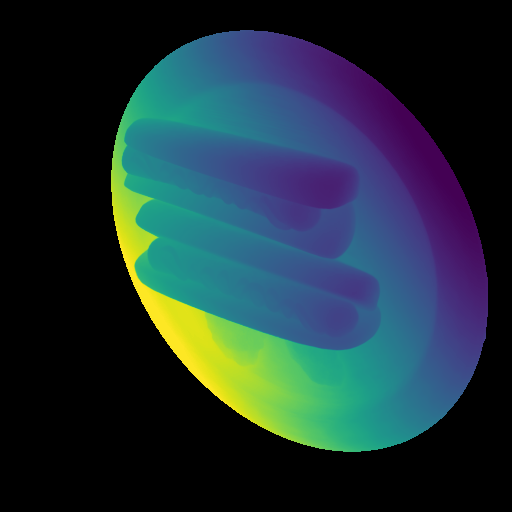
\includegraphics[width=1.22cm,height=1.22cm]{figures/decomp_hotdog/atlas_depth.png}};
\node[thumb] at (5.86,4.92) {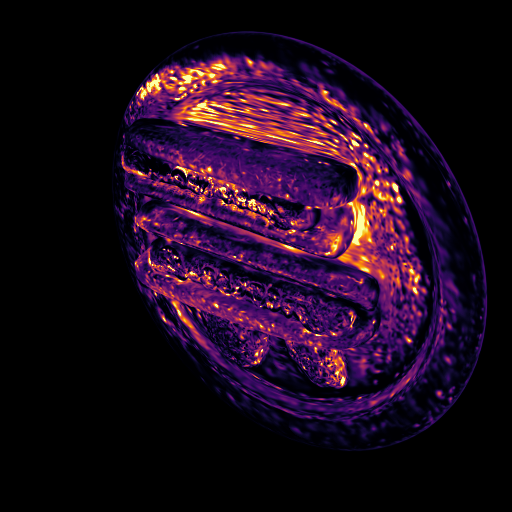
\includegraphics[width=1.22cm,height=1.22cm]{figures/decomp_hotdog/atlas_flux.png}};
\node[align=center] at (3.93,4.08) {depth $M_1,M_2$};
\node[align=center] at (5.86,4.08) {flux $\boldsymbol\Phi$};
\node at (4.91,3.72) {$\mathbf A(u)=\sum_i w_i(u)\,[\boldsymbol\phi_i,\,z_i,\,z_i^2,\,1]$};

\draw[lightflow] (6.88,4.92) -- (7.55,4.92);
\node[align=center] at (7.21,4.52) {blur\\$\downarrow 2$};
\node[title,anchor=south] at (8.50,5.62) {Pyramid $\{\mathbf A_k\}_{k<K}$};
\node[thumb] at (8.25,4.95) {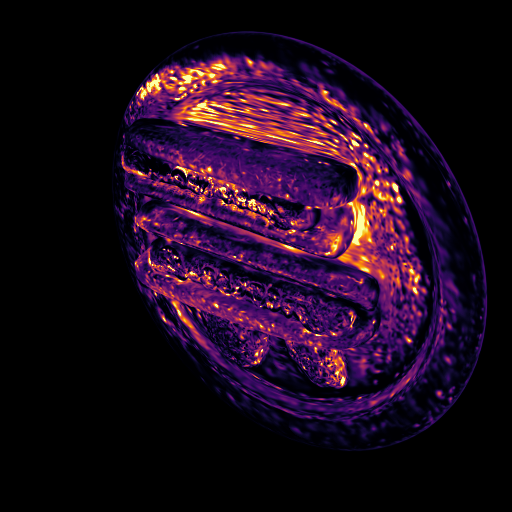
\includegraphics[width=1.22cm,height=1.22cm]{figures/decomp_hotdog/atlas_flux.png}};
\node[thumb] at (8.70,4.66) {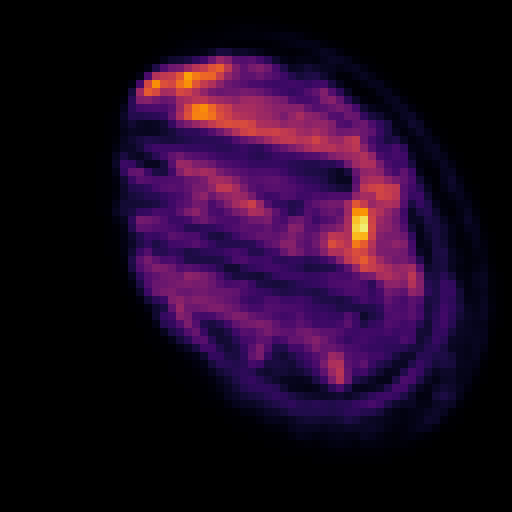
\includegraphics[width=0.90cm,height=0.90cm]{figures/decomp_hotdog/atlas_flux_level3.png}};
\node[thumb] at (9.06,4.42) {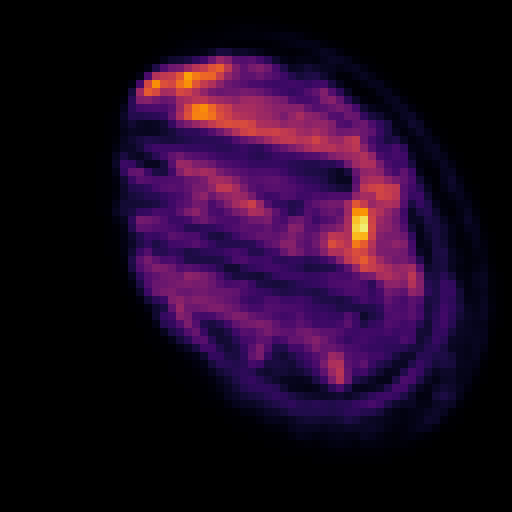
\includegraphics[width=0.62cm,height=0.62cm]{figures/decomp_hotdog/atlas_flux_level3.png}};

% ---------------------------------------------------------------- camera pass
\node[title,anchor=west,text=blue!60!black] at (0.05,3.38) {Camera pass};
\node[camera,minimum width=2.40cm,minimum height=1.20cm,align=center] (receivers) at (1.30,2.42)
  {\textbf{Receivers $\mathbf x$}\\[2pt]Gaussian centers (II)\\or pixels (III)};
\node[camera,minimum width=5.90cm,minimum height=1.20cm,inner sep=2pt,align=center] (gather) at (6.02,2.42)
  {\textbf{Gather at $u(\mathbf x)$, every level $k$}\\[2pt]
   $\mathbf q_k=[M_{0,k},\,t_k,\,\delta_k,\,\log\eta_k,\,V_k],\ \ \boldsymbol\Phi_k$\\[2pt]
   $V_k=1-M_{0,k}\,G(t_k-\beta)$};
\draw[cameraflow] (receivers.north) -- (1.30,3.24) -- (7.90,3.24) -- (7.90,4.32);
\node[label] at (4.85,3.24) {project into the light: $(u(\mathbf x),z(\mathbf x))$};
\draw[cameraflow] (8.70,4.20) -- (8.70,3.03);
\node[label,anchor=west] at (8.78,3.62) {sample};

% ---------------------------------------------------------------- learned heads
\node[title,anchor=west,text=green!45!black] at (10.05,6.18) {Shading};
\node[learned,minimum width=4.85cm,minimum height=1.05cm,align=center] (visibility) at (12.50,5.42)
  {\textbf{visibility $\mathcal G$}\\[2pt]$V=\sigma\big(\mathrm{logit}\,V_0+\mathcal G(\mathbf Q,\mathbf f,\mathbf n\!\cdot\!\mathbf l)\big)$};
\node[learned,minimum width=4.85cm,minimum height=1.05cm,align=center] (transfer) at (12.50,4.14)
  {\textbf{transfer $\mathcal K$}\\[2pt]$L_{\mathrm{tr}}=\sum_k\mathbf W_k\,\boldsymbol\Phi_k$, \ $\mathbf W_k$ from $\mathbf Q$};
\node[learned,minimum width=4.85cm,minimum height=1.05cm,align=center] (material) at (12.50,2.86)
  {\textbf{local material}\\[2pt]$\rho=\mathrm{MLP}(\mathbf f,\mathbf n,\mathbf l,\mathbf v,\mathbf h,\mathbf r)$, lobes $s$};
\draw[draw=blue!60!black] (gather.east) -- (9.70,2.42) -- (9.70,5.42);
\draw[cameraflow] (9.70,5.42) -- (visibility.west);
\draw[cameraflow] (9.70,4.14) -- (transfer.west);
\draw[cameraflow] (9.70,2.86) -- (material.west);
\fill[blue!60!black] (9.70,4.14) circle (0.65pt);
\fill[blue!60!black] (9.70,2.86) circle (0.65pt);

\node[thumb] (visimage) at (16.20,5.42) {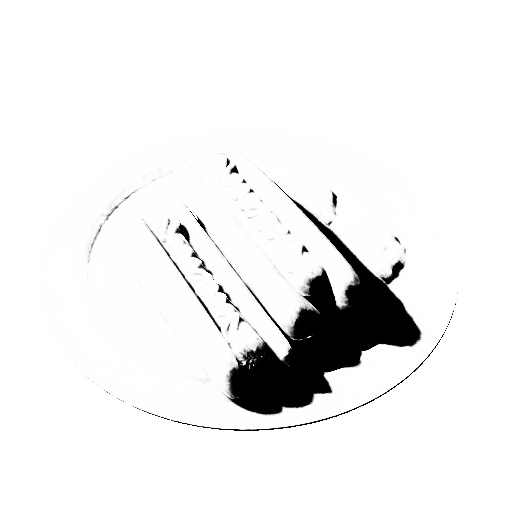
\includegraphics[width=1.12cm,height=1.12cm]{figures/decomp_hotdog/visibility.png}};
\node[thumb] (trimage) at (16.20,4.14) {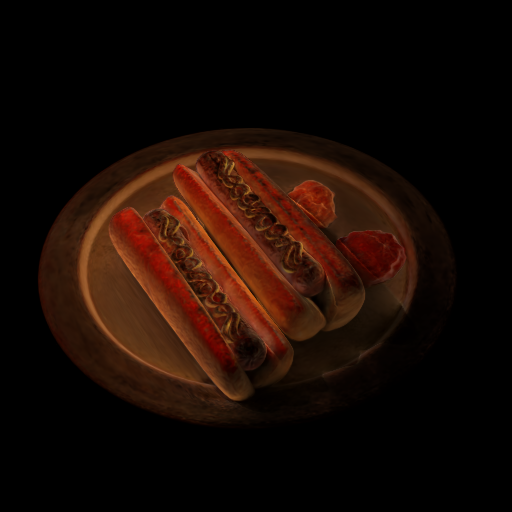
\includegraphics[width=1.12cm,height=1.12cm]{figures/decomp_hotdog/transfer.png}};
\node[thumb] (matimage) at (16.20,2.86) {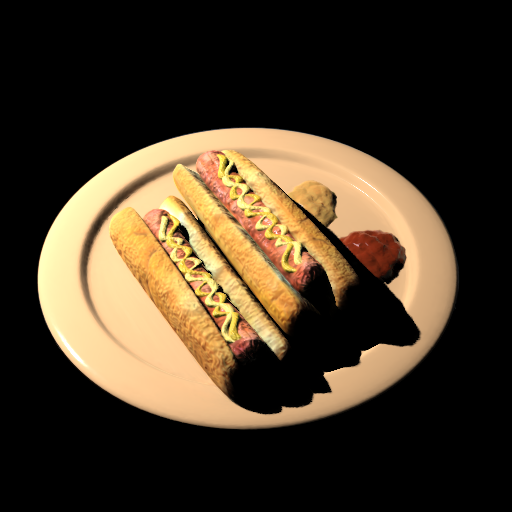
\includegraphics[width=1.12cm,height=1.12cm]{figures/decomp_hotdog/local.png}};
\draw[draw=green!45!black] (visibility.east) -- (visimage.west);
\draw[draw=green!45!black] (transfer.east) -- (trimage.west);
\draw[draw=green!45!black] (material.east) -- (matimage.west);

% ---------------------------------------------------------------- radiance
\draw[draw=black!75] (15.25,5.42) -- (15.25,2.03);
\fill[black!75] (15.25,5.42) circle (0.65pt);
\fill[black!75] (15.25,4.14) circle (0.65pt);
\fill[black!75] (15.25,2.86) circle (0.65pt);
\node[draw=black,fill=white,rounded corners=2pt,minimum width=15.0cm,minimum height=0.58cm,align=center] (shading) at (7.62,1.45)
  {$L(\mathbf x)=\bar E(\mathbf x)\big[\,V\rho+V_0\,s+\textstyle\sum_k\mathbf W_k\boldsymbol\Phi_k\big],\qquad \bar E(\mathbf x)=\mathbf I/\|\mathbf p-\mathbf x\|^2$};
\draw[mergeflow] (15.25,2.03) -- (15.25,1.74);
\node[thumb] (output) at (16.55,1.45) {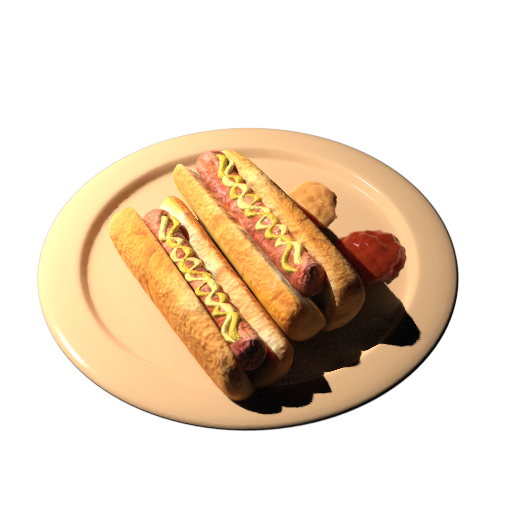
\includegraphics[width=1.05cm,height=1.05cm]{figures/decomp_hotdog/ours.png}};
\draw[mergeflow] (shading.east) -- (output.west);

% ---------------------------------------------------------------- schedule (8k : 22k : 8k)
\fill[gray!10] (0.06,0.02) rectangle (3.7116,0.98);
\fill[blue!8] (3.7116,0.02) rectangle (13.7534,0.98);
\fill[green!8] (13.7534,0.02) rectangle (17.405,0.98);
\draw[draw=gray!60,rounded corners=2pt] (0.06,0.02) rectangle (17.405,0.98);
\draw[draw=gray!60] (3.7116,0.02) -- (3.7116,0.98);
\draw[draw=gray!60] (13.7534,0.02) -- (13.7534,0.98);
\node[stage,text width=3.50cm] at (0.16,0.90)
  {\textbf{I. Geometry warm-up} (8k)\\no networks; target $Y^{1/\gamma}\!\to\!Y$};
\node[stage,text width=9.80cm] at (3.84,0.90)
  {\textbf{II. Joint training} (22k)\\linear-radiance loss; Gaussian receivers; densification};
\node[stage,text width=3.55cm] at (13.86,0.90)
  {\textbf{III. Refinement} (8k)\\frozen geometry; pixel receivers; display-domain loss};
\end{tikzpicture}
}
  \caption{\textbf{Overview.}
For every light, the Gaussians are rasterized once from the light; each deposits learned flux features $\boldsymbol\phi_i$ and its depth moments with the compositing weight that equals the fraction of light it intercepts (\cref{eq:atlas}).
A receiver projects into the light, gathers multi-scale statistics and flux from the pyramid, and is shaded by a residual on the moment shadow test, transfer kernels applied linearly to the gathered flux features, and a local material.
Thumbnails: actual buffers of our Hotdog model on a test view. Bottom: the schedule of \cref{sec:optimization}.}
  \label{fig:pipeline}
\end{figure*}


We reconstruct an object from images $\{Y_m\}$, each taken by a calibrated camera under a point light at $\vect p_m$ with RGB intensity $\vect I_m$ (\cref{fig:pipeline}).

\subsection{Preliminaries}
\label{sec:prelim}
The scene is a set of 3D Gaussians with means $\mu_i$, covariances $\Sigma_i$ and opacities $o_i$~\cite{kerbl20233d}, each carrying a base color $\vect b_i\in\mathbb R^3$ and a latent material code $\vect f_i\in\mathbb R^{32}$ whose first three channels define a learned unit normal $\vect n_i$.
Splatting composites per-Gaussian attributes $\vect c_i$ front to back,
\begin{equation}
  \bar{\vect c}(u)=\sum_i w_i(u)\,\vect c_i,\qquad w_i(u)=\alpha_i(u)\prod_{j<i}\big(1-\alpha_j(u)\big),
  \label{eq:composite}
\end{equation}
where $\alpha_i(u)$ is the opacity of Gaussian $i$ at pixel $u$.
For a point $\vect x$ we write $\vect l,\vect v,\vect h$ for the unit light, view and half vectors and $\bar E(\vect x)=\vect I/\|\vect p-\vect x\|^2$ for the irradiance at normal incidence.

\subsection{Splatting from the light records the deposit}
\label{sec:deposit}
Place a perspective camera at the light, aimed at the scene center, with a field of view that covers the splatted extent of 99.9\% of the Gaussians.
Its pixel $u$ subtends a solid angle $d\omega_u$ and receives the flux $\vect I\,d\omega_u$.
Splatting treats each Gaussian as absorbing the fraction $\alpha_i(u)$ of the light still travelling along the ray, so the flux it intercepts is
\begin{equation}
  P_i(u)=\vect I\,d\omega_u\,w_i(u),
  \label{eq:flux}
\end{equation}
with the weights of \cref{eq:composite}.
This holds within the rasterized splatting model, whose per-tile sorting by center depth, low-pass filter and clamped opacities approximate volumetric transmittance~\cite{radl2024stopthepop,huang2024error,talegaonkar2025volumetrically,yu2024mip}.
No normal or distance enters \cref{eq:flux}: since an element $dA$ at distance $r$ and incidence $\theta$ receives $\vect I\cos\theta\,dA/r^2=\vect I\,d\omega$, foreshortening and falloff are accounted for by how many light pixels a surface covers.

\paragraph{Atlas.}
Every Gaussian emits $\vect c_i=[\boldsymbol\phi_i,\,z_i,\,z_i^2,\,1]$, where $z_i$ is the depth of its center along the light's axis relative to the scene center, normalized by the scene radius, and $\boldsymbol\phi_i=\softplus(\mathrm{MLP}_\phi(\vect f_i,\vect b_i,\vect n_i\cdot\vect l_i))\in\mathbb R_+^{C}$ are $C=8$ learned flux features.
One rasterization at $512^2$ yields the atlas
\begin{equation}
  \vect A(u)=\sum_i w_i(u)\,\vect c_i=\big[\boldsymbol\Phi(u),\,M_1(u),\,M_2(u),\,M_0(u)\big],
  \label{eq:atlas}
\end{equation}
the deposit per unit of the pixel's incident flux: $M_0$ is the fraction of that flux absorbed by the scene, $M_1/M_0$ and $M_2/M_0$ are the first two moments of the depth at which it is absorbed, and $\boldsymbol\Phi$ describes what it hit.
The absolute deposit $\vect I\,d\omega_u\vect A(u)$ also involves $d\omega_u\propto\cos^3$ of the off-axis angle, which varies by less than 30\% across a typical atlas in our data (up to $2.1\times$ at the corners of the widest one); the shadow statistics below are ratios that do not depend on it, and the transfer term ignores it.
A pyramid $\vect A_0,\dots,\vect A_{K-1}$ with $K=7$ follows from repeated binomial blurring and $2\times$ decimation.
Because every channel is linear in the weights $w_i$, each level still holds moments and feature sums of the deposit, over footprints growing from one texel to about a third of the object, which is what makes such shadow maps filterable~\cite{donnelly2006variance,peters2015moment}.

\subsection{Shading from the atlas}
\label{sec:shading}
A receiver $\vect x$ projects into the light view at $u(\vect x)$ with normalized depth $z(\vect x)$ and samples every level bilinearly.
At level $k$ we form the mean deposit depth $\bar z_k=M_{1,k}/M_{0,k}$, a spread $\eta_k=(M_{2,k}/M_{0,k}-\bar z_k^2+\tau_k^2)^{1/2}$ that includes the texel size $\tau_k$, the offset $\delta_k=z-\bar z_k$ of the receiver behind the deposit, and $t_k=\delta_k/\eta_k$.
If the depth of the deposit within a footprint were normally distributed, the fraction of light absorbed in front of the receiver would be $M_{0,k}\,G(t_k)$ with the standard normal CDF $G$, which gives the moment test
\begin{equation}
  V_k=1-M_{0,k}\,G(t_k-\beta),
  \label{eq:moment}
\end{equation}
where the bias $\beta=3$, in units of the local spread, prevents self-shadowing.
The descriptors $\vect q_k=[M_{0,k},t_k,\delta_k,\log\eta_k,V_k]$ of all levels form $\vect Q(\vect x)\in\mathbb R^{5K}$.
The test is a weak prior where an occluder and the receiver share a footprint (for a half-transparent occluder in front of an opaque receiver, $t_0=1$ and \cref{eq:moment} returns $0.98$ instead of $0.5$, which the Chebyshev bound of variance shadow maps gets right~\cite{donnelly2006variance}), and each Gaussian deposits the depth of its center, so a large, obliquely lit Gaussian appears at a single depth.

\paragraph{Visibility.}
A residual network $\mathcal G$, initialized to zero, corrects the finest test,
\begin{equation}
  V(\vect x)=\sigma\big(\logit V_0(\vect x)+\mathcal G(\vect Q,\vect f,\vect n\cdot\vect l)\big),
  \label{eq:visibility}
\end{equation}
so training starts from a classical filtered shadow map, and $\mathcal G$ learns from the multi-scale statistics to repair the cases above, the partial transmittance of fur and the soft shadow boundaries of real, finite lights.

\paragraph{Transfer.}
By \cref{eq:flux}, light that enters a translucent object and leaves it at $\vect x$ contributes $\vect I\!\int\!\sum_i R(\vect x,\mu_i)\,w_i(\omega)\,d\omega$: a receiver-dependent kernel $R$ integrated against the deposit over the light's solid angle.
Translucent shadow maps evaluate such integrals with stored irradiance and fixed diffusion kernels~\cite{dachsbacher2003translucent,deon2007efficient,jimenez2010real}.
We learn both the deposited features and the kernels, using the pyramid levels as kernels of increasing width:
\begin{align}
  L_{\mathrm{tr}}(\vect x)&=\textstyle\sum_{k}\vect W_k\,\boldsymbol\Phi_k(\vect x),\label{eq:transfer}\\
  \{\vect W_k\}_k&=\softplus\big(\mathcal K(\vect Q,\vect f,\vect n\cdot\vect l,\vect n\cdot\vect v)\big),\quad \vect W_k\in\mathbb R_+^{3\times C}.\nonumber
\end{align}
The kernels depend only on the receiver and the geometric statistics $\vect Q$, so for a given geometry and light $L_{\mathrm{tr}}$ is linear in the deposited features; since the receiver's own deposit lies in its footprint, nothing prevents $L_{\mathrm{tr}}$ from also absorbing part of the direct reflection, and the split between the terms is learned.

\paragraph{Local material and radiance.}
The local reflectance $\rho(\vect x)$ is a latent-code neural BRDF: an MLP of $\vect f$, $\vect n$, Fourier encodings of $\vect l,\vect v,\vect h$ and the reflected view direction $\vect r$, their cosines and highlight hints $e^{\kappa(\vect n\cdot\vect h-1)}$~\cite{zeng2023nrhints}, times a smoothed cosine $\psi(\vect n\cdot\vect l)=\softplus(20\,\vect n\cdot\vect l)/20$.
Position enters only through eight light-independent coefficients that mix eight light-dependent responses, which limits how much cast shadow can be baked into the material (the free per-Gaussian codes still allow some), and isotropic lobes $s(\vect x)$ with fixed sharpness $\kappa\in\{8,\dots,2048\}$ and light-independent weights carry sharp highlights.
The outgoing radiance is
\begin{equation}
  L(\vect x)=\bar E(\vect x)\big[V(\vect x)\,\rho(\vect x)+V_0(\vect x)\,s(\vect x)+L_{\mathrm{tr}}(\vect x)\big].
  \label{eq:radiance}
\end{equation}
The lobes use the geometric test $V_0$, so highlights keep a gradient path where the learned $V$ is still wrong.
Factoring $\bar E(\vect x)$ out lets the networks predict reflectance-like quantities; for $L_{\mathrm{tr}}$ it replaces the falloff at the entry points by that at the receiver, which is off by the squared ratio of their light distances, $(r_{\mathrm{out}}/r_{\mathrm{in}})^2$, for back-lit transmission; the kernels can absorb this only on average, which suffices when light distances vary little within a capture (constant in the synthetic scenes, within $1.8\times$ in the real ones; supplement).
All inputs of $\mathcal G$ and $\mathcal K$ are relative to the light, so the operator is defined in the light's frame rather than indexed by its position; whether this helps extrapolation is the subject of experiment E1 (\cref{sec:exp_atlas}).

\subsection{Receivers: Gaussians or pixels}
\label{sec:receivers}
\emph{Gaussian receivers} shade every Gaussian center $\mu_i$ and composite the colors with \cref{eq:composite}; \emph{pixel receivers} composite $\vect b,\vect f$ and the expected depth first, lift each pixel to a world point and shade it once.
Gaussian receivers give the geometry the ordinary rasterization gradients that densification relies on and keep overlapping surfaces from mixing materials, but they inherit the per-primitive shadow limitation of \cref{sec:intro}.
Pixel receivers evaluate the shadow test at each pixel's own surface point, so a shadow boundary can cross a large Gaussian.
Like RNG's switch from forward to deferred shading~\cite{fan2025rng}, \ours uses Gaussian receivers while the geometry is optimized and pixel receivers once it is fixed (\cref{sec:optimization}), with the same atlas.
